\chapter[Code instructions]{Code instructions}

\begin{chapabstract}
    A Python implementation of the above-mentioned frameworks is available on the INRIA \href{https://gitlab.inria.fr/aldabyse/hidenn_1d}{Gitlab}.
\end{chapabstract}

\minitoc

\section{Implementation of a HiDeNN for a 1D Bar}

The objective of this code is to provide an implementation of a HiDeNN. The layer's input is the coordinate $\vect{x}$ where the output is evaluated. In this case, the output of the network is the displacement $\vect{u}\left(\vect{x}\right)$

The first hidden layers play the role of linear shape functions by applying constraints on the weights and bias of sub-networks composing the first layers. The last hidden layer called the interpolation layer in the remainder of the document, utilises the output of the shape functions to interpolate the output. Training the weights of that last hidden layer is the same as solving a FEM problem on a fixed mesh. The weights of the interpolation layer directly correspond to the nodal values associated with each shape function. Therefore, prescribing Dirichlet boundary conditions is straightforward by freezing the weights associated with the prescribed values of fixed DoFs.

\subsection{Architecture of the NN}


\begin{itemize}
    \item Linear left and right classes that are the two elementary blocks to create a linear 1D shape function
   \item Shape class that are based on the two aforementioned building blocks and, given an index, build the shape function associated with that index i
   \item MeshNN class that, given geometric parameters, "assemble" the shape functions accordingly
    \begin{itemize}
        \item \code{model = MeshNN(np,L)}
        \item np \& L being the number of DoFs and the length of the bar, respectively
   \end{itemize}
   \item The Dirichlet boundary conditions (BCs) are set by calling
   \begin{itemize}
        \item \code{model.setBCs(u\_0,u\_L)} 
        \item with $u_0$ and $u_L$ being the prescribed displacement at $x=0$ and $x=L$ respectively
        \end{itemize}
\end{itemize}

\subsection{Training the NN }

The Volumic forces are accounted for in the loss function through the right-hand side (RHS) function, and the loss function is the potential energy.

The trainable parameters can be changed on the fly. 
\begin{itemize}
    \item \code{model.Freeze\_Mesh()} Freezes the mesh so that only the nodal values are trained
    \item \code{model.UnFreeze\_Mesh()} Unfreezes the mesh so that the coordinates values can be trained
    \item \code{model.Freeze\_FEM()} Freezes the nodal values so that only the coordinates are trained
    \item \code{model.UnFreeze\_FEM()} Unfreezes the nodal so that the FEM problem can be solved
\end{itemize}


\section{Parser}

As usually done in a Finite element (FE) framework, interpolating the quantities of interest in the spatial domain is achieved using shape functions associated with a mesh.
\Rq{The difference being that the input and output are ``post-processed'' in the sense that the underlying mesh is invisible to the user. Another difference is that the mesh used to initialise the HiDeNN is not fixed and can be adapted throughout the training process. Only the external nodes of the mesh, describing the structure's geometry, are fixed to conserve the structural shape of the strudied object.}

In order to convert information from the mesh to the HiDeNN architecture, a parser is required.

\subsection{Mesh format}
This parser relies on the \code{.msh} format exported in the \code{Mesh.MshFileVersion = 2.2}.


\section{Implementations}

\Rq{Note that the assembly matrix (just as the assembled stiffness matrix in a FE code) is not created through for loops but in a vectorised way so as to minimise overhead costs.}


The shape functions in 1D are sorted so that the in an element the node associated to the left part of a shape function is above the node associated to the right part of the shape function. 
Note that this lead to the two part of the shape functions not to be adjacent in the output intermediate layer. as illustrated in \cref{fig:SortingSF}.

\begin{figure}
    \centering
    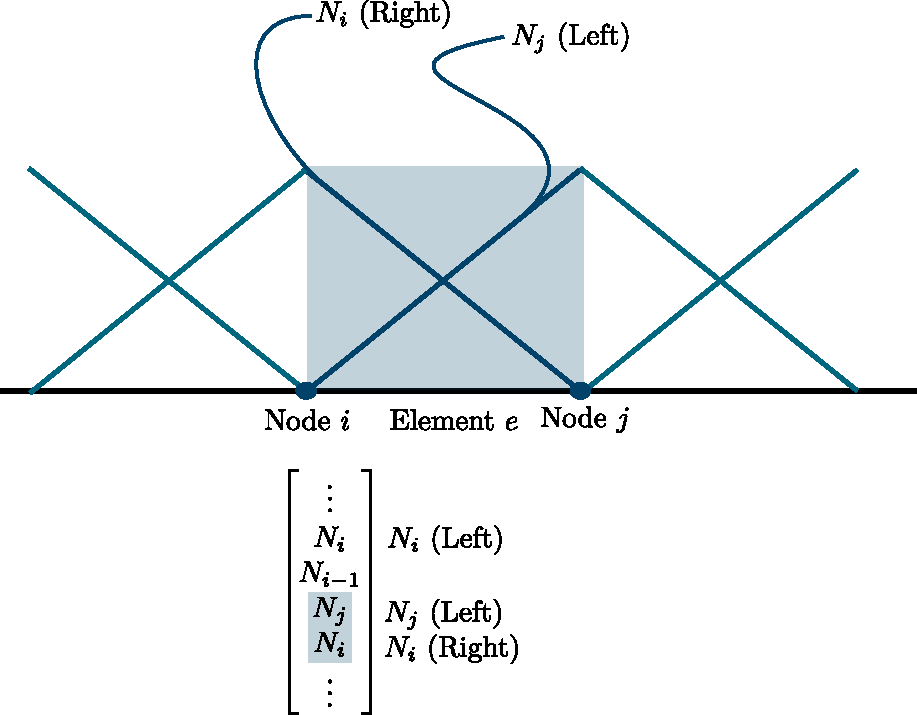
\includegraphics[width = 0.7\linewidth]{Figures/SortingOfShapeFunctions.pdf}
    \caption{Sorting of the shape functions in each element}
    \label{fig:SortingSF}
\end{figure}